%% CHAPTER 14 COMPLEX NUMBERS -- dictated by Maximus (26 Oct 2026); more to come
\clearpage
\inchap{Complex Numbers}
\section{Cartesian Form}
\begin{definition}{Cartesian form of a complex number}
Every complex number $z\in\mathbb{C}$ can be expressed as $z=x+y\mathrm{i}$, $x,y\in\mathbb{R}$.
\begin{itemize}
\item A complex number $z$ is \textbf{real} if $\operatorname{Im}(z)=0$.
\item A complex number $z$ is \textbf{purely imaginary} if $\operatorname{Re}(z)=0$ \fhl{and $\operatorname{Im}(z)\neq0$}.
\end{itemize}
\end{definition}
\section{Complex Number Arithmetic}
\begin{itemize}
\item \textbf{Addition \& subtraction}: similar to surds.
\item \textbf{Multiplication}: similar to surds.
\item \textbf{Division}: similar to surds, remember to \textit{realise}.
\item \textbf{Square roots} (See Example 14.1)
\end{itemize}
\exlab
Find the values of $\sqrt{3+4\mathrm{i}}$. \fhl{\sidenote{(or, solve for $z^{2}=3+4\mathrm{i}$)}}
\cdisp{(a+b\mathrm{i})^{2}&=3+4\mathrm{i}\\a^{2}-b^{2}+2ab\,\mathrm{i}&=3+4\mathrm{i}}
By comparing real \& imaginary parts,
\cdisp{a^{2}-b^{2}=3,\quad2ab&=4\\&\;\;\vdots\\a=2,\ b=1\text{ or }a=-2,\ b&=-1\\\therefore\sqrt{3+4\mathrm{i}}=2+\mathrm{i}\text{ or }&-2-\mathrm{i}}
\begin{theorem}{Equality of Complex Numbers}
Two complex numbers $z_{1}=a_{1}+b_{1}\mathrm{i}$ and $z_{2}=a_{2}+b_{2}\mathrm{i}$ are equal if and only if their real parts are equal and their imaginary parts are equal.
\[z_{1}=z_{2}\iff a_{1}=a_{2}\text{ and }b_{1}=b_{2}\]
This is basically comparing \textbf{real} and \textbf{imaginary} parts.
\end{theorem}
\section{Simultaneous Equations}
\textbf{Common types:}
\begin{enumerate}
\item Standard $z$, $w$ (no conjugate, no modulus, no square)
\cdisp{2z+w&=2-4\mathrm{i}\\\mathrm{i}z-w&=2\mathrm{i}}
\item With $z^{*}$ and $w$ (or vice versa, or both)
\cdisp{z+2z^{*}+w=6+\mathrm{i}\quad\text{and}\quad\mathrm{i}z-w=3}
\hfill{\small[MI 2025 Prelim P2 Q3(a)]}\par
{\color{gray}If both $z^{*}$ and $w^{*}$ are in the equation, it is still solvable. Consider this example: $z=2+\mathrm{i}w\Rightarrow z^{*}=2-\mathrm{i}w^{*}$}
\item With $z^{2}$ and $w$
\cdisp{\fhlm{z^{2}}-\mathrm{i}w+2&=0\\\fhlm{z}&=w+\mathrm{i}+3}
\hfill{\small[NYJC 2024 Prelim P1 Q1]}\par
{\color{gray}The quadratic formula is useful here; avoid letting $z=a+b\mathrm{i}$ and expanding, though it works.}
\item With $z$ and $|w|$
\cdisp{z+w^{*}+5\mathrm{i}=10\quad\text{and}\quad\left|w\right|^{2}=z+18+\mathrm{i}}
\hfill{\small[CJC 2017 Prelim P2 Q4(a)]}\par
{\color{gray}For $w=a+b\mathrm{i}$, $\left|w\right|=\sqrt{a^{2}+b^{2}}$.}
\end{enumerate}
\begin{info}[title=Note]
Please check your answers using your GC for \textbf{BOTH} equations! The answers are usually quite nice and not ugly numbers.
\end{info}
\clearpage
\section{Polynomials}
\begin{theorem}{Complex Conjugate Root Theorem}
If all the coefficients of a polynomial equation $\mathrm{P}(z)=0$ are real, and $z=\alpha$ is a root, then its conjugate $z=\alpha^{*}$ is also a root.
\end{theorem}

\exlab
{\small[ACJC/2014/I/4]}\par\noindent
\begin{tabular}{@{}p{0.7cm}p{0.88\linewidth}@{}}
(i)&Given that $1+\mathrm{i}$ is a root of the equation $2w^{3}+aw^{2}+bw-2=0$, find the values of the real numbers $a$ and $b$.\hfill[4]\\
(ii)&For these values of $a$ and $b$, solve the equation in part \textbf{\fhl{(i)}}, without the use of a calculator.\hfill[3]
\end{tabular}\par
{\setlength{\columnseprule}{0.4pt}\begin{multicols}{2}
\noindent\textbf{Method 1: Apply CCRT}
\cdisp{w&=1+\mathrm{i}\text{ is a root}\\\therefore w&=1-\mathrm{i}\text{ is a root}\\\left(w-(1+\mathrm{i})\right)\left(w-(1-\mathrm{i})\right)&=(w-1)^{2}-\mathrm{i}^{2}\\&=w^{2}-2w+2\\2w^{3}+aw^{2}+bw-2&=\left(w^{2}-2w+2\right)(Aw+B)\\w^{3}:\quad A&=2\\w^{0}:\quad2B&=-2\\B&=-1\\Aw+B=2w-1&=0\\\therefore w&=\frac12\\w^{2}:\quad a&=B-2A=-5\\w^{1}:\quad b&=2A-2B=6\\\therefore a=-5,\ b&=6\\\therefore w=1+\mathrm{i},\ 1-\mathrm{i},\ &\tfrac12}
\columnbreak
\noindent\textbf{Method 2: Substitute the root}
\cdisp{2(1+\mathrm{i})^{3}+a(1+\mathrm{i})^{2}+b(1+\mathrm{i})-2&=0\\(b-6)+(2a+b+4)\mathrm{i}&=0}
By comparing real \& imaginary parts,
\cdisp{b-6=0,\quad2a+b+4&=0}
\fhlp{\cdisp{\therefore a=-5,\ b&=6\\w&=1+\mathrm{i}\text{ is a root}\\\therefore w&=1-\mathrm{i}\text{ is a root}\\\left(w-(1+\mathrm{i})\right)\left(w-(1-\mathrm{i})\right)&=w^{2}-2w+2\\2w^{3}-5w^{2}+6w-2&=\left(w^{2}-2w+2\right)(Aw+B)\\&\;\;\vdots}
{\centering\color{gray}\small(compare coefficients or long divide)\par}
\cdisp{&\;\;\vdots\\A=2,\ B&=-1\\\therefore w=1+\mathrm{i},\ 1-\mathrm{i},\ &\tfrac12}}
\end{multicols}}
\begin{info}[title=Note]
If you see a really weird question you have never seen before, you can try letting the complex number $=a+b\mathrm{i}$ as a last resort and see where you get with it (unless it becomes unreasonably tedious).
\end{info}
\clearpage
\exlab
{\small[RI Promo/9758/2018/Q11(a)(ii)]} It is given that one of the roots of the equation $z^{3}-(1+4\mathrm{i})z^{2}-(3-9\mathrm{i})z+(14-2\mathrm{i})=0$ is purely imaginary. Find all the roots of the equation, giving your answers in Cartesian form $a+\mathrm{i}b$.\hfill[6]\par
{\color{gray}The coefficients are not all real, so the Complex Conjugate Root Theorem does not apply.}
\cdisp{\text{Let }z&=k\mathrm{i},\ k\in\mathbb{R}\\-k^{3}\mathrm{i}+(1+4\mathrm{i})k^{2}-(3-9\mathrm{i})k\mathrm{i}+14-2\mathrm{i}&=0\\\left(k^{2}-9k+14\right)+\left(-k^{3}+4k^{2}-3k-2\right)\mathrm{i}&=0}
By comparing real \& imaginary parts,
\cdisp{k^{2}-9k+14=0,\quad-k^{3}+4k^{2}-3k-2&=0\\(k-2)(k-7)&=0\\k&=2\text{ or }7\\k=2:\quad-8+16-6-2&=0\\k=7:\quad-343+196-21-2&\neq0\\\therefore k&=2,\quad z=2\mathrm{i}}
\cdisp{{\color{blue}z^{3}-(1+4\mathrm{i})z^{2}-(3-9\mathrm{i})z+(14-2\mathrm{i})}&{\color{blue}=(z-2\mathrm{i})\left(Az^{2}+Bz+C\right)}}
{\color{gray}Here, $A,B,C\in\mathbb{C}$, so we cannot compare real and imaginary parts for an equation involving $A$, $B$ or $C$.}
\cdisp{z^{3}:\quad A&=1\\z^{2}:\quad B-2\mathrm{i}A&=-1-4\mathrm{i}\\B&=-1-2\mathrm{i}\\z^{0}:\quad-2\mathrm{i}C&=14-2\mathrm{i}\\C&=1+7\mathrm{i}\\z^{2}-(1+2\mathrm{i})z+(1+7\mathrm{i})&=0\\z&=\frac{(1+2\mathrm{i})\pm\sqrt{(1+2\mathrm{i})^{2}-4(1+7\mathrm{i})}}{2}\\&=\frac{(1+2\mathrm{i})\pm{\color{red}\sqrt{-7-24\mathrm{i}}}}{2}\quad\text{\color{gray}(use GC here!)}\\&=\frac{(1+2\mathrm{i})\pm(3-4\mathrm{i})}{2}\\\therefore z=2\mathrm{i},\ 2-\mathrm{i},\ &-1+3\mathrm{i}}

{\color{gray}This question does not say ``without using a calculator'', so use your GC to evaluate anything you can, instead of expanding things out manually.}




\clearpage
\section{Argand Diagram}
\subsection{Modulus}
\begin{definition}{Modulus of a Complex Number}
The \textbf{Modulus} of complex number, or absolute value, is defined as:
\[|z|=|a+b\mathrm{i}|=\sqrt{a^{2}+b^{2}}.\]
\end{definition}
It is represented by the distance from the origin, to the coordinate represented by the complex number in an Argand diagram.

\noindent\textbf{Properties of Modulus}\par
Let $z=a+b\mathrm{i}$ and $w=x+y\mathrm{i}$, where $a,b,x,y\in\mathbb{R}$. Then we have the following useful properties.
\begin{center}\begin{tabular}{@{}p{0.46\linewidth}p{0.46\linewidth}@{}}$\bullet$\ $|z|^{2}=a^{2}+b^{2}$. (Obviously)&$\bullet$\ $|z^{*}|=|z|$.\end{tabular}\\[10pt]
\begin{tabular}{@{}p{0.31\linewidth}p{0.31\linewidth}p{0.31\linewidth}@{}}{\color{gray}$\bullet$\ $|zw|=|z||w|$.}&{\color{gray}$\bullet$\ $\left|\dfrac{z}{w}\right|=\dfrac{|z|}{|w|}$.}&{\color{gray}$\bullet$\ $|z^{n}|=|z|^{n}$.}\end{tabular}\end{center}









{\color{gray}You are not required to memorise the last 3 formulas in the 'A' Level syllabus, but may be asked to show them and use it in a question.}

\subsection{Argument}
\begin{definition}{Argument of a Complex Number}
An \textbf{argument} of the complex number $z=x+\mathrm{i}y$, denoted $\arg(z)$, is defined geometrically, as the 2D polar angle $\theta$ from the positive real axis to the vector representing $z$.
\end{definition}
\begin{info}[title=Note]
The argument, $\theta$, of all complex numbers must lie within the range $-\pi<\theta\le\pi$.
\end{info}
Given a complex number, to find its argument,\par
\textbf{Step 1:} find basic angle $\alpha=\tan^{-1}\left|\dfrac{b}{a}\right|$.\par
\textbf{Step 2:} draw a small Argand diagram to figure out which quadrant it is in based on its coordinate. (e.g. $-1+\sqrt3\,\mathrm{i}\iff(-1,\sqrt3)$ is in the 2nd quadrant)
\newcommand{\argd}[3]{\begin{tikzpicture}[scale=0.8,>=stealth]
\draw[->](-1.6,0)--(1.8,0)node[right]{\scriptsize Re};\draw[->](0,-1.6)--(0,1.8)node[above]{\scriptsize Im};
\node[below left]at(0,0){\scriptsize$O$};
\draw[thick](0,0)--(#1,#2);\fill(#1,#2)circle(1.5pt);#3\end{tikzpicture}}
\begin{center}
\renewcommand{\arraystretch}{1.4}\begin{tabular}{|*{4}{>{\centering\arraybackslash}m{\dimexpr0.25\linewidth-2\tabcolsep-1pt\relax}|}}\hline
\textbf{1st Quadrant}&\textbf{2nd Quadrant}&\textbf{3rd Quadrant}&\textbf{4th Quadrant}\\\hline
\argd{1.2}{1.2}{\draw(0.5,0)arc(0:45:0.5);\node at(0.75,0.28){\tiny$\alpha$};}&
\argd{-1.2}{1.2}{\draw(-0.5,0)arc(180:135:0.5);\node at(-0.75,0.28){\tiny$\alpha$};}&
\argd{-1.2}{-1.2}{\draw(-0.5,0)arc(180:225:0.5);\node at(-0.75,-0.28){\tiny$\alpha$};}&
\argd{1.2}{-1.2}{\draw(0.5,0)arc(0:-45:0.5);\node at(0.75,-0.28){\tiny$\alpha$};}\\\hline
$\arg(z)=\alpha$&$\arg(z)=\pi-\alpha$&$\arg(z)=-(\pi-\alpha)$&$\arg(z)=-\alpha$\\\hline
\end{tabular}\renewcommand{\arraystretch}{1}
\end{center}
\cautionbox[Caution]{For purely real or imaginary numbers, it is recommended to find the argument of them via considering their position on the Argand diagram.}
\begin{center}
\begin{tabular}{cccc}
\argd{1.3}{0}{\node[above]at(1.3,0){\scriptsize$5$};}&
\argd{-1.3}{0}{\node[above]at(-1.3,0){\scriptsize$-5$};\draw[->,red](0.45,0)arc(0:180:0.45);}&
\argd{0}{1.3}{\node[right]at(0,1.3){\scriptsize$\mathrm{i}$};\draw[->,red](0.5,0)arc(0:90:0.5);}&
\argd{0}{-1.3}{\node[right]at(0,-1.3){\scriptsize$-\mathrm{i}$};\draw[->,red](0.5,0)arc(0:-90:0.5);}\\
$\arg(5)=0$&$\arg(-5)=\pi$&$\arg(\mathrm{i})=\dfrac{\pi}{2}$&$\arg(-\mathrm{i})=-\dfrac{\pi}{2}$
\end{tabular}
\end{center}

\noindent\textbf{Properties of Argument}\par
Let $\arg(z)=\theta_{z}$ and $\arg(w)=\theta_{w}$. Then we have the following useful properties.
\begin{center}$\bullet$\ $\arg(z^{*})=-\arg(z)$.\\[10pt]
\begin{tabular}{@{}p{0.31\linewidth}p{0.31\linewidth}p{0.31\linewidth}@{}}{\color{gray}$\bullet$\ $\arg(zw)=\arg(z)+\arg(w)$\newline\hspace*{1em}$=\theta_{z}+\theta_{w}$.}&{\color{gray}$\bullet$\ $\arg\left(\dfrac{z}{w}\right)=\arg(z)-\arg(w)$\newline\hspace*{1em}$=\theta_{z}-\theta_{w}$.}&{\color{gray}$\bullet$\ $\arg(z^{n})=n\cdot\arg(z)=n\theta_{z}$.}\end{tabular}\end{center}








{\color{gray}You are not required to memorise the last 3 formulas in the 'A' Level syllabus, but they may be given to you and you have to use them to answer the rest of the question.}

\clearpage
\subsection{Finding Cartesian Form Given Modulus and Argument}
\exlab
{\small[ASRJC 2025 Prelims P2 Q6]} The point $Q$ is represented by the complex number $q$, where \[\arg(q)=\frac{2}{3}\pi\quad\text{and}\quad|q|=2.\]\par\noindent
\begin{tabular}{@{}p{0.7cm}p{0.88\linewidth}@{}}
(a)&Sketch the point $Q$ on an Argand diagram.\hfill[2]\\
(b)&Use the Argand diagram to deduce $\operatorname{Re}(q)$ and $\operatorname{Im}(q)$, giving your answers in exact form.\hfill[2]
\end{tabular}\par
\begin{center}
\begin{tikzpicture}[scale=1.1,>=stealth]
\draw[->](-2,0)--(1.5,0)node[right]{\small Re};\draw[->](0,-0.4)--(0,2.2)node[above]{\small Im};
\node[below right]at(0,0){\small$O$};
\draw[thick](0,0)--(-1,1.732)node[midway,above right]{\small$2$};\fill(-1,1.732)circle(1.6pt)node[left]{\small$Q$};
\draw[->,red](0.4,0)arc(0:120:0.4);\node[red]at(0.55,0.5){\small$\tfrac{2\pi}{3}$};
\end{tikzpicture}\qquad\qquad
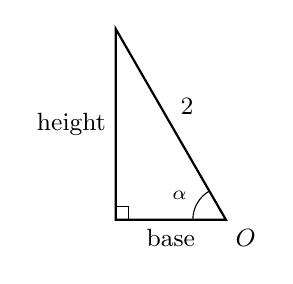
\begin{tikzpicture}[scale=1.4]
\draw[thick](0,0)--(-1,0)--(-1,1.732)--cycle;
\draw(-1,0)rectangle(-0.88,0.12);
\node[above right]at(-0.5,0.87){\small$2$};\node[below]at(-0.5,0){\small base};\node[left]at(-1,0.87){\small height};
\draw(-0.3,0)arc(180:120:0.3);\node at(-0.42,0.22){\scriptsize$\alpha$};\node[below right]at(0,0){\small$O$};
\end{tikzpicture}
\end{center}
\cdisp{\alpha&=\pi-\frac{2\pi}{3}=\frac{\pi}{3}\\\text{base}&=2\cos\frac{\pi}{3}=1\\\text{height}&=2\sin\frac{\pi}{3}=\sqrt3\\\therefore\operatorname{Re}(q)&=-1,\quad\operatorname{Im}(q)=\sqrt3}
{\color{gray}$Q$ is in the 2nd quadrant, so the real part is negative.}
\cautionbox[Common Mistake]{Let $q=a+b\mathrm{i}$,
\cdisp{\sqrt{a^{2}+b^{2}}=2,\quad\tan^{-1}\frac{b}{a}=\frac{2\pi}{3}\quad\textcolor{red}{\text{\ding{55}\ding{55}}}}
{\color{gray}This is very tedious to solve, and the argument equation is also wrong; we can't simply take $\tan^{-1}\frac{b}{a}$ to find the argument for any complex number. We need to first find the basic angle then consider which quadrant it is in.}}

\clearpage
\subsection{Addition and Scalar Multiplication in an Argand Diagram}
Complex numbers in an Argand diagram behave like 2 dimensional vectors. When adding two complex numbers (vectors) together, the result follows the parallelogram law of vector addition. Similarly, multiplying a complex number (vector) by a scalar constant scales its length, and if the scalar is negative, it reflects the complex number (vector) about the origin.
\exlab
{\small[Modified from ASRJC 2025 Prelims P2 Q6]} The points $P$, $Q$ and $R$ correspond to the complex numbers $p$, $q$ and $p+q$ respectively. Given $p=\sqrt2+\sqrt2\,\mathrm{i}$, $q=-1+\sqrt3\,\mathrm{i}$.\par\noindent
\begin{tabular}{@{}p{0.7cm}p{0.88\linewidth}@{}}
(a)&Sketch $P$, $Q$ and $R$ on a single Argand diagram.\\
(b)&By considering $\arg(p+q)$ or otherwise, show that $\tan\left(\dfrac{11}{24}\pi\right)=\sqrt6+\sqrt3+\sqrt2+2$.\hfill[3]
\end{tabular}\par
\textbf{(a)}


\noindent\begin{minipage}[c]{0.55\linewidth}\centering
\begin{tikzpicture}[scale=1.0,>=stealth]
\draw[->](-2,0)--(2.4,0)node[right]{\small Re};\draw[->](0,-0.4)--(0,3.6)node[above]{\small Im};
\node[below right]at(0,0){\small$O$};
\draw[thick,blue](0,0)--(1.414,1.414)node[midway,below right]{\small$2$};\fill[blue](1.414,1.414)circle(1.6pt)node[right]{\small$P\,(p)$};
\draw[thick,red](0,0)--(-1,1.732)node[midway,below left]{\small$2$};\fill[red](-1,1.732)circle(1.6pt)node[left]{\small$Q\,(q)$};
\draw[dashed](1.414,1.414)--(0.414,3.146)--(-1,1.732);
\draw[thick,green!45!black](0,0)--(0.414,3.146);\fill[green!45!black](0.414,3.146)circle(1.6pt)node[above right]{\small$R\,(p+q)$};
\draw[->,blue](0.7,0)arc(0:45:0.7);\node[blue]at(0.95,0.32){\small$\tfrac{\pi}{4}$};
\draw[->,red](0.35,0)arc(0:120:0.35);\node[red]at(-0.45,0.38){\small$\tfrac{2\pi}{3}$};
\end{tikzpicture}
\end{minipage}\hfill\begin{minipage}[c]{0.42\linewidth}{\color{gray}Note: $p+q=\left(\sqrt2-1\right)+\left(\sqrt2+\sqrt3\right)\mathrm{i}$\par\medskip Here, we use vector addition to determine the position of $R$, rather than its coordinate $\left(\sqrt2-1,\ \sqrt2+\sqrt3\right)$.}\end{minipage}\par

\textbf{(b)}\par
{\color{gray}$|p|=|q|=2$, so $OPRQ$ is a rhombus and $OR$ bisects angle $POQ$.}
\cdisp{\because|p|=|q|&=2\\\arg(p+q)&=\frac12\left(\frac{\pi}{4}+\frac{2\pi}{3}\right)=\frac{11\pi}{24}}
By TOA CAH SOH,\par
\noindent\begin{minipage}[c]{0.36\linewidth}\centering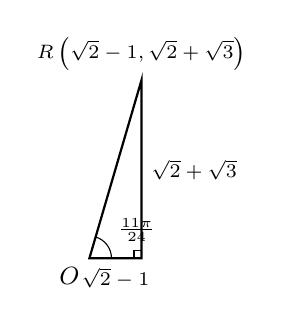
\begin{tikzpicture}[scale=0.8]\draw[thick](0,0)--(0.414*2,0)--(0.414*2,3.146*0.9)--cycle;\draw(0.828,0)rectangle(0.708,0.12);\node[below left]at(0,0){\small$O$};\node[below]at(0.414,0){\scriptsize$\sqrt2-1$};\node[right]at(0.828,1.4){\scriptsize$\sqrt2+\sqrt3$};\node[above]at(0.828,2.83){\scriptsize$R\left(\sqrt2-1,\sqrt2+\sqrt3\right)$};\draw(0.35,0)arc(0:73.7:0.35);\node at(0.75,0.45){\scriptsize$\frac{11\pi}{24}$};\end{tikzpicture}\end{minipage}\begin{minipage}[c]{0.62\linewidth}\cdisp{\tan\left(\frac{11\pi}{24}\right)&=\frac{\sqrt2+\sqrt3}{\sqrt2-1}\\&=\frac{\left(\sqrt2+\sqrt3\right)\left(\sqrt2+1\right)}{\left(\sqrt2-1\right)\left(\sqrt2+1\right)}\\&=2+\sqrt2+\sqrt6+\sqrt3\\\therefore\tan\left(\frac{11\pi}{24}\right)&=\sqrt6+\sqrt3+\sqrt2+2\quad\text{(shown)}}\end{minipage}

\subsection{Transformations on the Argand Diagram}
\newcommand{\trd}[5]{\begin{tikzpicture}[scale=1.0,>=stealth]\useasboundingbox(-2.1,-2.0)rectangle(2.7,2.3);
\draw[->](-1.8,0)--(1.9,0)node[right]{\scriptsize Re};\draw[->](0,-1.7)--(0,1.8)node[above]{\scriptsize Im};
\node[below left]at(0,0){\scriptsize$O$};
\draw[thick,blue](0,0)--(1.2,0.7);\fill[blue](1.2,0.7)circle(1.5pt)node[above right]{\small$z$};
\draw[thick,red](0,0)--(#1,#2);\fill[red](#1,#2)circle(1.5pt)node[#3]{\small$#4$};#5
\end{tikzpicture}}
\begin{center}
\renewcommand{\arraystretch}{1.3}
\begin{tabular}{|>{\centering\arraybackslash}m{2.9cm}|>{\centering\arraybackslash}m{5.4cm}|>{\centering\arraybackslash}m{4.6cm}|}\hline
\textbf{Transformation}&\textbf{Diagram}&\textbf{Description}\\\hline
$z\to z^{*}$&\trd{1.2}{-0.7}{below right}{z^{*}}{\draw[blue](0.6,0)arc(0:30.3:0.6);\node[blue]at(0.85,0.22){\scriptsize$\theta$};\draw[red](0.6,0)arc(0:-30.3:0.6);\node[red]at(0.85,-0.22){\scriptsize$\theta$};}&Reflect about real axis\\\hline
$z\to-z$&\trd{-1.2}{-0.7}{below left}{-z}{\draw[blue](0.5,0)arc(0:30.3:0.5);\node[blue]at(0.72,0.2){\scriptsize$\theta$};\draw[->,red](0.8,0)arc(0:-149.7:0.8);\node[red]at(0.6,-0.95){\scriptsize$-\pi+\theta$};}&Reflect about origin\\\hline
$z\to\mathrm{i}z$&\trd{-0.7}{1.2}{above left}{\mathrm{i}z}{\draw($(0,0)!0.25!(1.2,0.7)$)--++(-0.7*0.25,1.2*0.25)--($(0,0)!0.25!(-0.7,1.2)$);\draw[->,red](1.1,0.98)arc(41.5:110:1.45);}&Rotate anticlockwise by $90^{\circ}$\\\hline
$z\to-\mathrm{i}z$&\trd{0.7}{-1.2}{below right}{-\mathrm{i}z}{\draw($(0,0)!0.25!(1.2,0.7)$)--++(0.7*0.25,-1.2*0.25)--($(0,0)!0.25!(0.7,-1.2)$);\draw[->,red](1.4,0.3)arc(12:-50:1.45);}&Rotate clockwise by $90^{\circ}$\\\hline
\end{tabular}
\end{center}
